\subsection{Hand Labeling of Independent Components}
Before the automatic FIX classifier could be used to identity components of noise and interest it needed to be trained with a set of hand labeled components \cite{Salimi-Khorshidi2014}. All 2500 components were manually hand labeled. \\
The process of the hand labeling followed that the investigators labeled half of the components each, where after the labeled components were cross-checked and discussed by the investigators. The investigator assessment relied heavily on information with regards to hand labeling provided by Griffanti et al. \cite{Griffanti2017} and Salimi-Khorshidi et al. \cite{Salimi-Khorshidi2014}. As a final assessment an expert in the field of fMRI did a control and corrected labels if they not did not fit the expert's opinion. \\
The MELODIC tool proposed a set of predefined classes to label the components as. The classes suited for noise were movement, susceptibility-motion, MRI, cardiac, respiratory, white matter, sagittal sinus and unclassified noise. It was possible that one component could contain more than one noise class. If all noise classes of the component were identifiable, more classes were added to the component. The unclassified noise class was proposed for components containing a mixture of different noise sources, which were less clear to pinpoint. A class named unknown was intended for labeling components that contained both noise and signal. For any signal of interest the signal class was proposed, as there was no discrimination between different types of signal of interest. 
The following illustrations \figref{fig:meth:Movement}, \figref{fig:meth:sus}, \figref{fig:meth:MRI}, \figref{fig:meth:phys}, \figref{fig:meth:walter_white}, \figref{fig:meth:sinus}, \figref{fig:meth:Unoise}, \figref{fig:meth:unknown} and \figref{fig:meth:signal} show transverse spatial examples (inferior to superior) of components related to the various noise classes, the signal class and the unknown class.

\begin{figure}[H]                 
	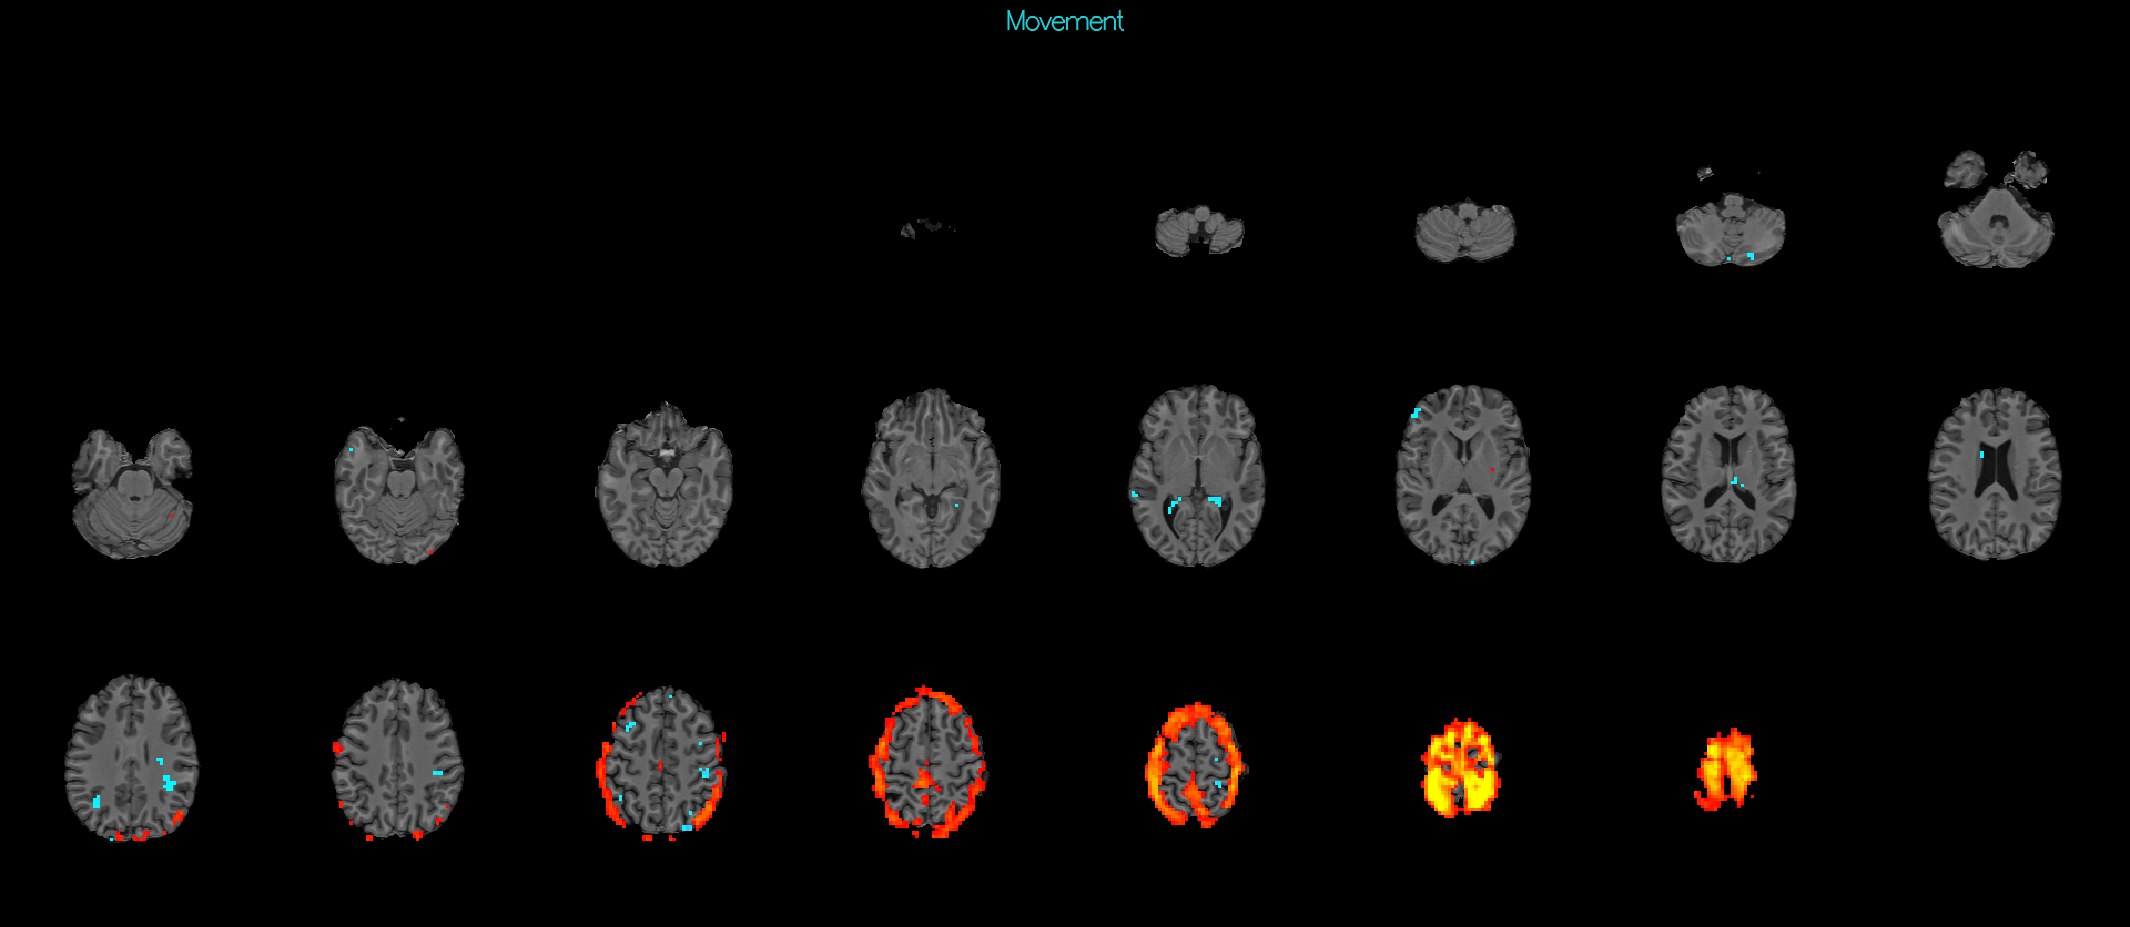
\includegraphics[width=.85\textwidth]{figures/bMethods/Movement}  
	\caption{An example component of the movement artefact. Movement noise will usually be seen as a ring or lines on the periphery of the brain. Depending on the nature of the movement causing the noise, the voxels will be located on the inside or outside of the brain.}
	\label{fig:meth:Movement} 
\end{figure}


\begin{figure}[H]                 
	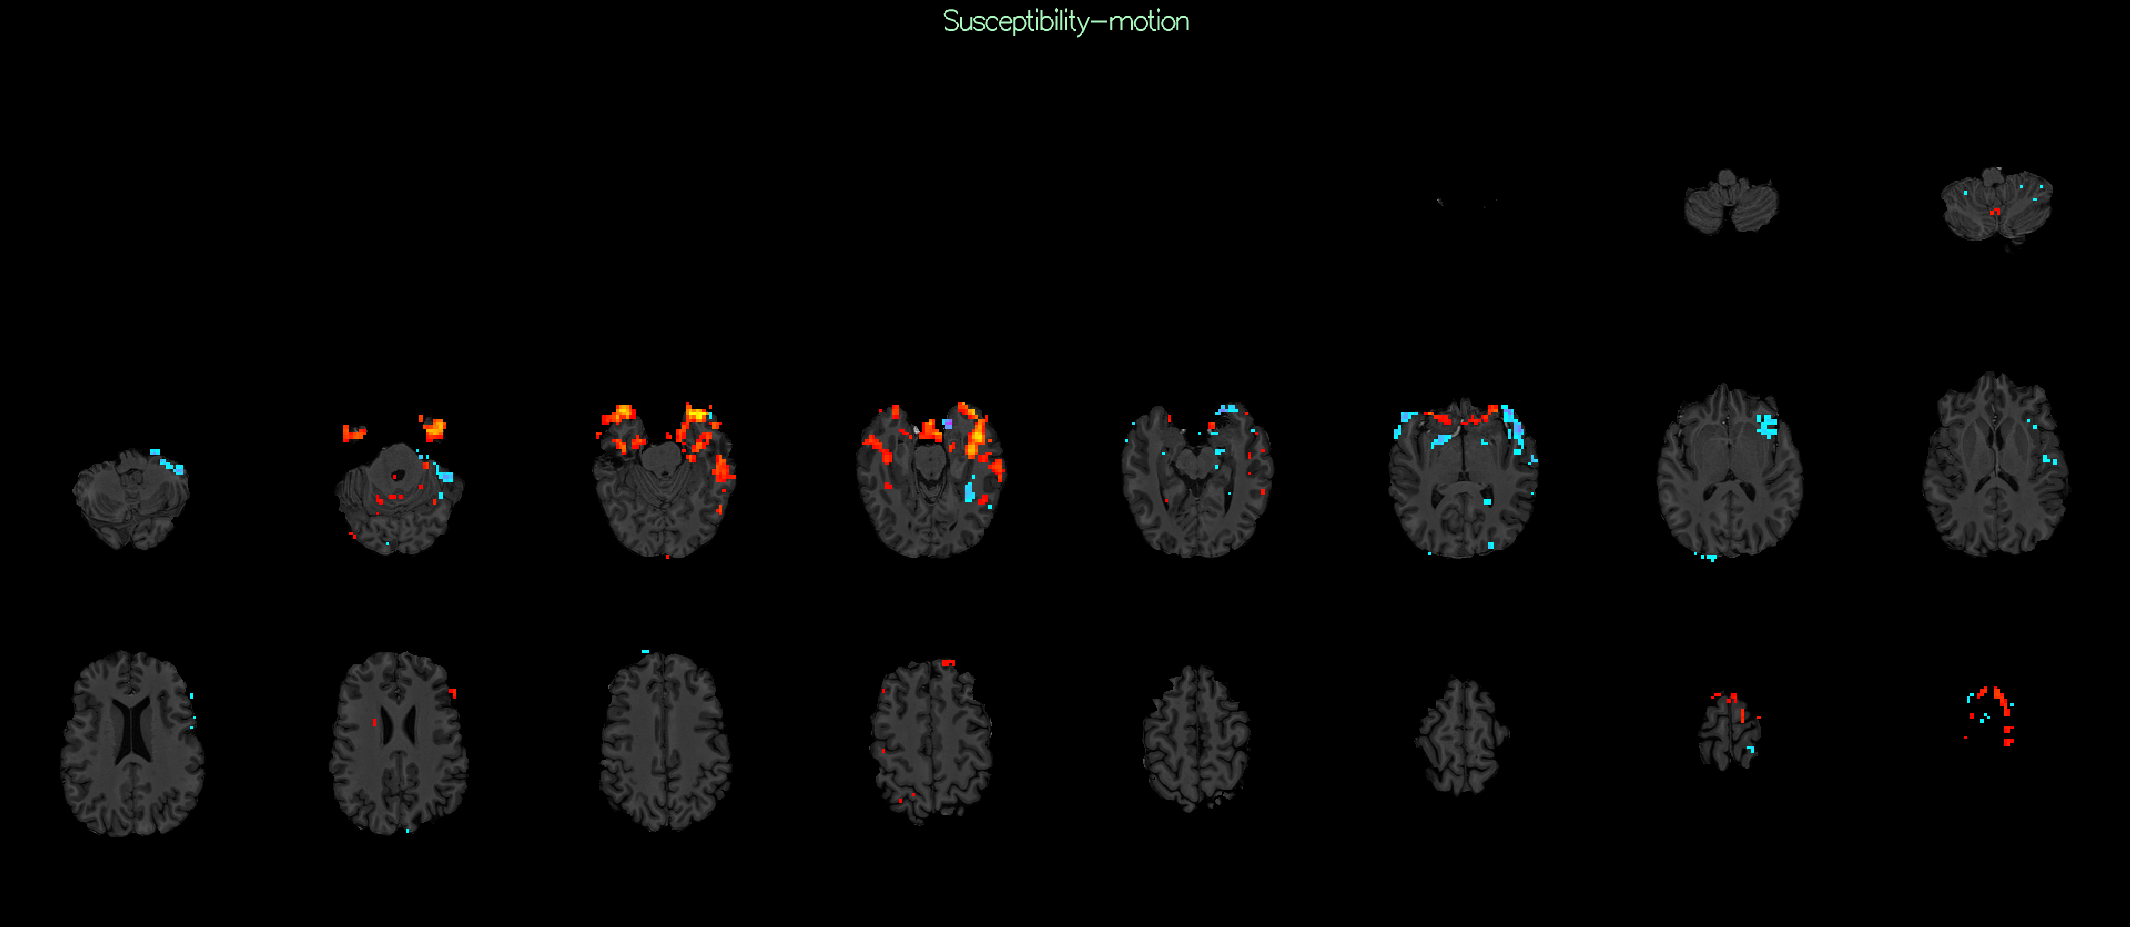
\includegraphics[width=.85\textwidth]{figures/bMethods/Susceptibility_motion}  
	\caption{An example component of the susceptibility-motion artefact. Susceptibility-motion noise is mainly due to air-tissue interfaces, and thus usually spatially expressed as a mix of activation and deactivation at the frontal sinuses.}
	\label{fig:meth:sus} 
\end{figure}

\begin{figure}[H]                 
	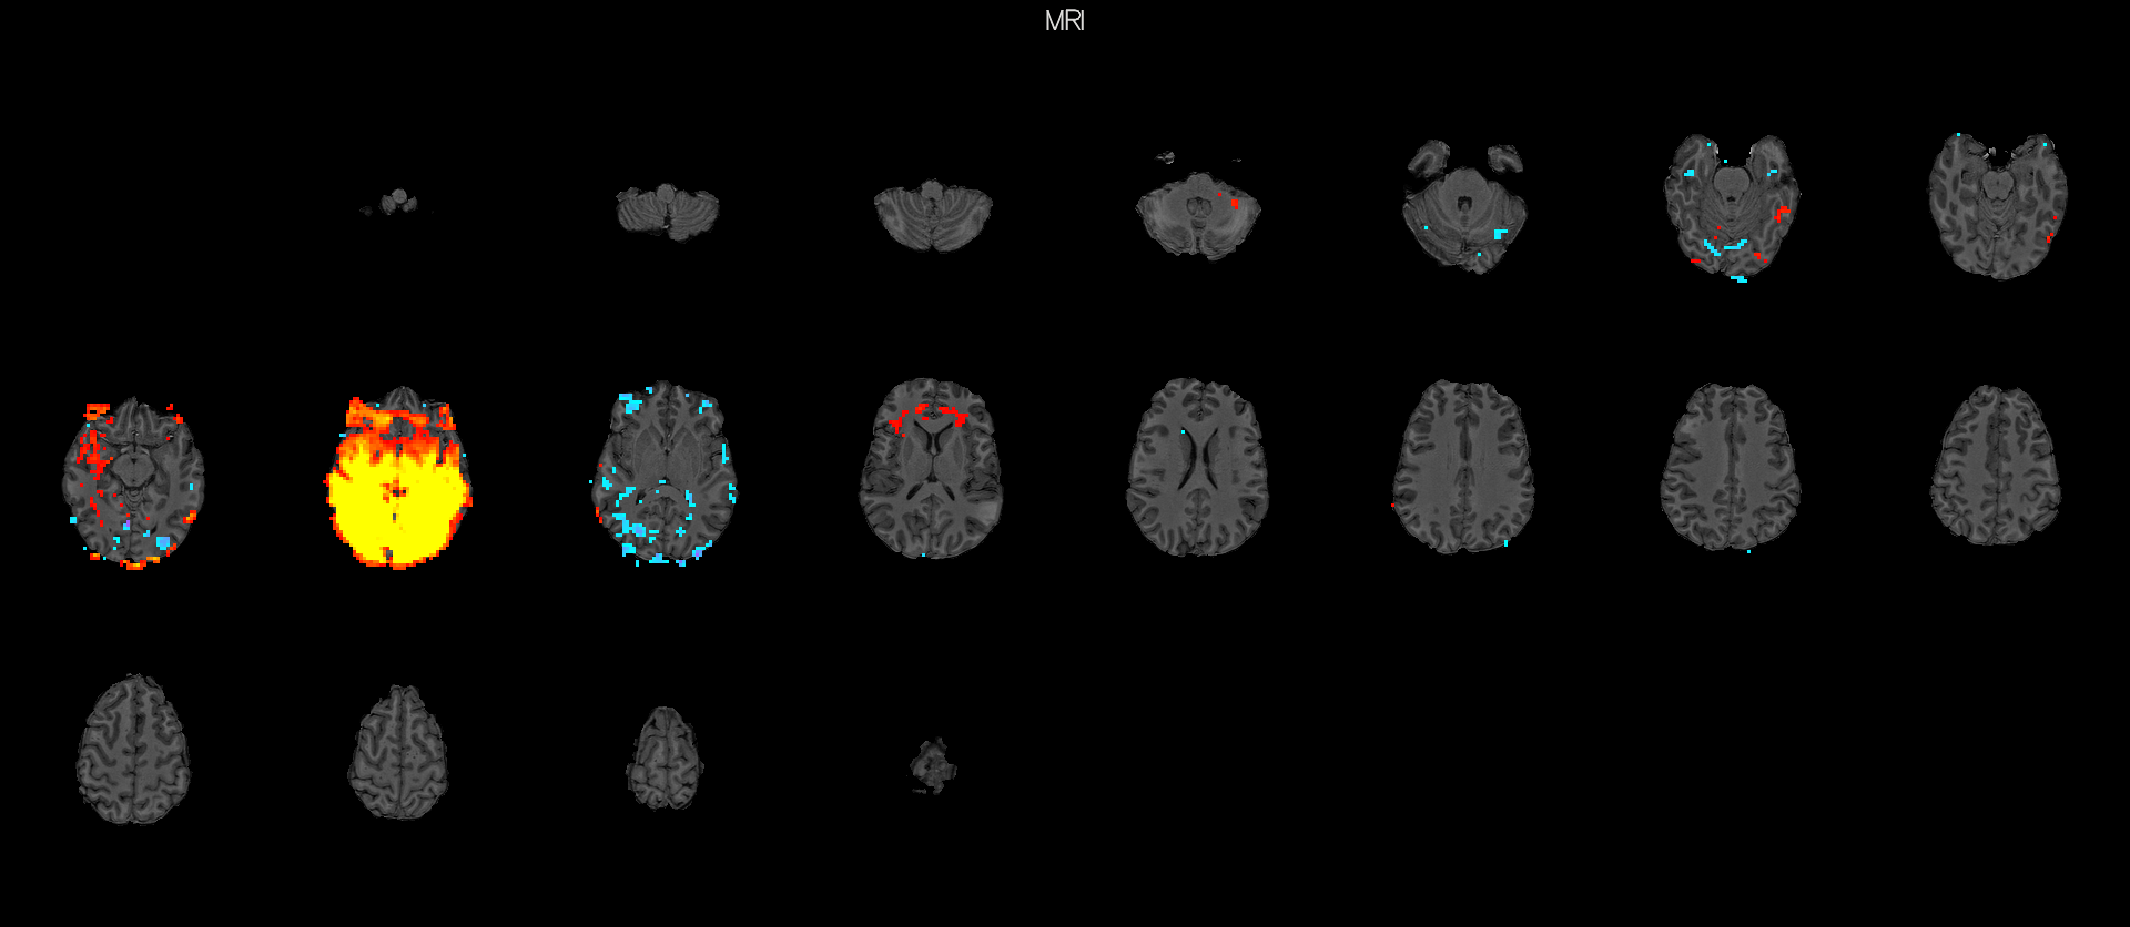
\includegraphics[width=.85\textwidth]{figures/bMethods/MRI}  
	\caption{An example component of the MRI artefact. This artefact is usually visualized as one or several fully activated or deactivated slices in separated spatial levels. In the sagittal or coronal plane, this is reflected as clear stripes in the images, which can not be explained as physiologically meaningful. Another example is slices containing large portions of alternating activation and deactivation, which too can not be physiologically explained.}
	\label{fig:meth:MRI} 
\end{figure}

\begin{figure}[H]                 
	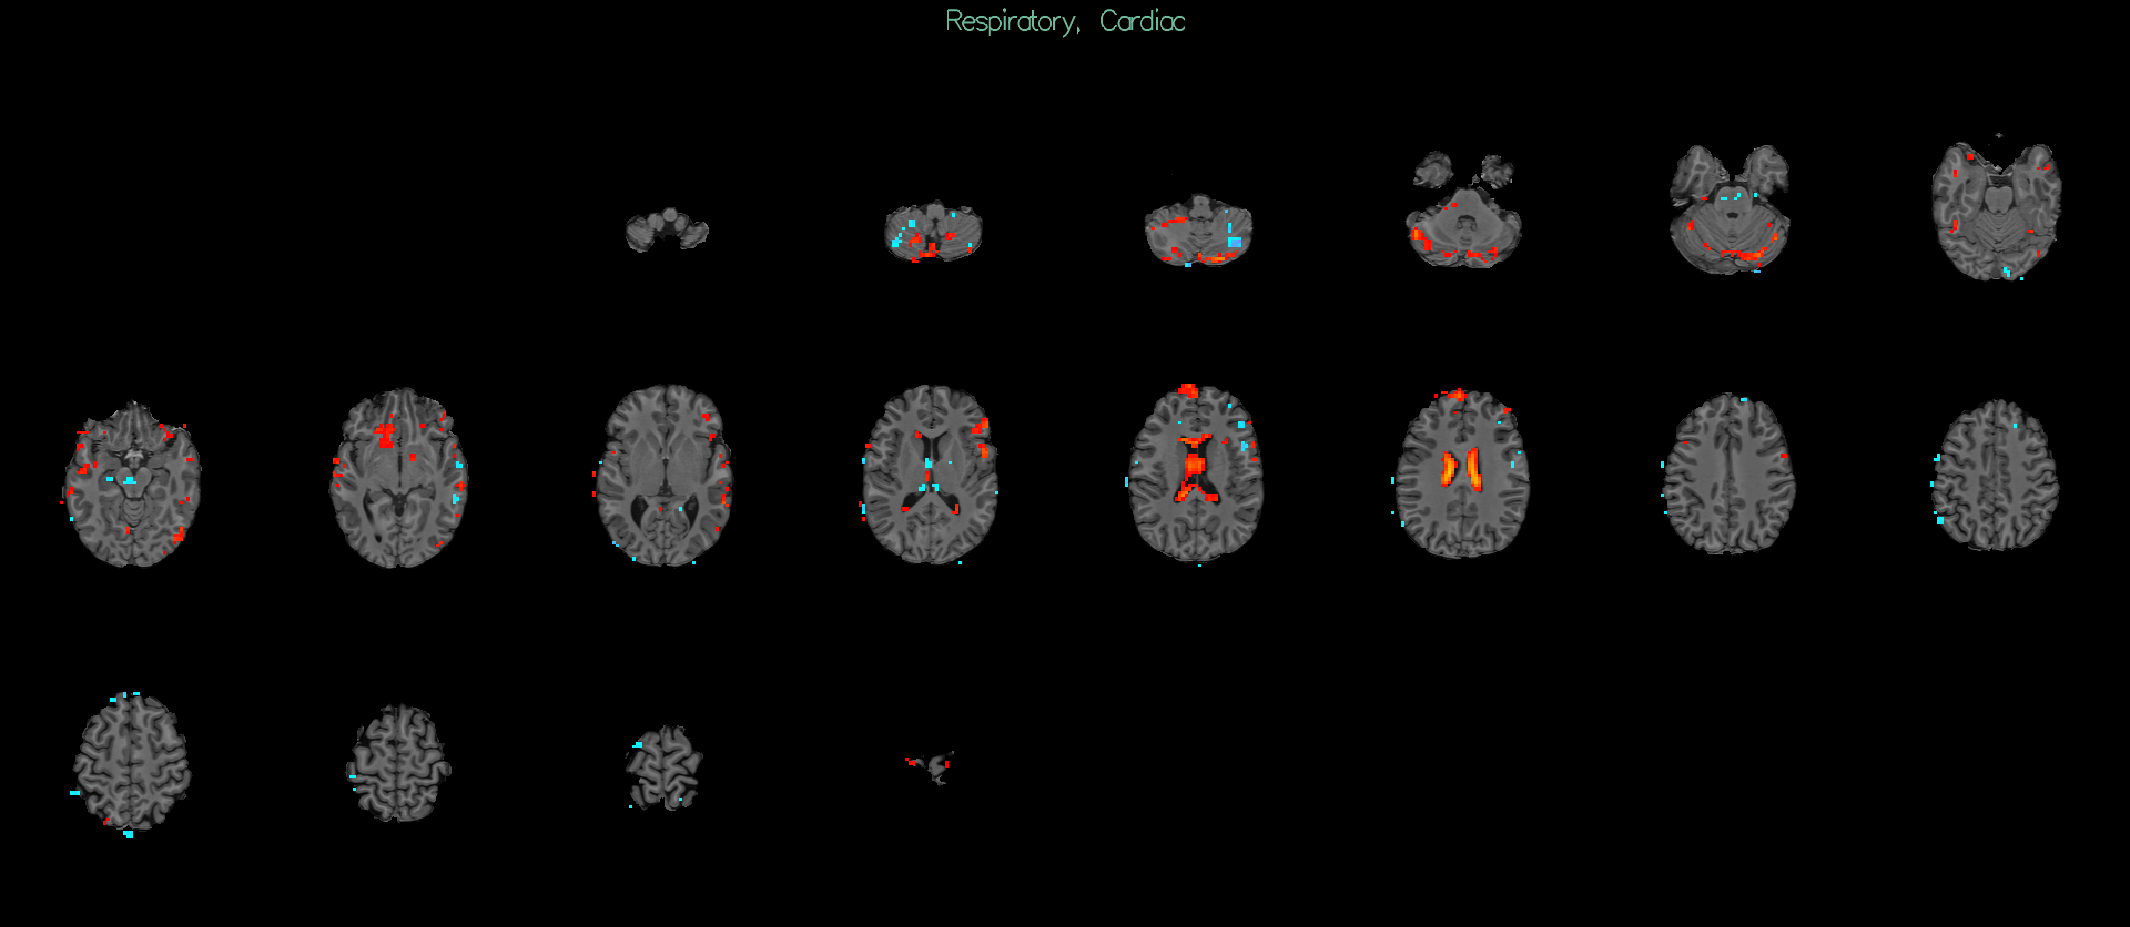
\includegraphics[width=.85\textwidth]{figures/bMethods/card_resp}  
	\caption{An example component of cardiac and respiratory artefacts. Cerebrospinal fluid pulsation is usually due to respiratory and cardiac cycles. Thus, activation of the ventricular system of the brain will be an indicator of respiratory and/or cardiac artefacts.}
	\label{fig:meth:phys} 
\end{figure}

\begin{figure}[H]                 
	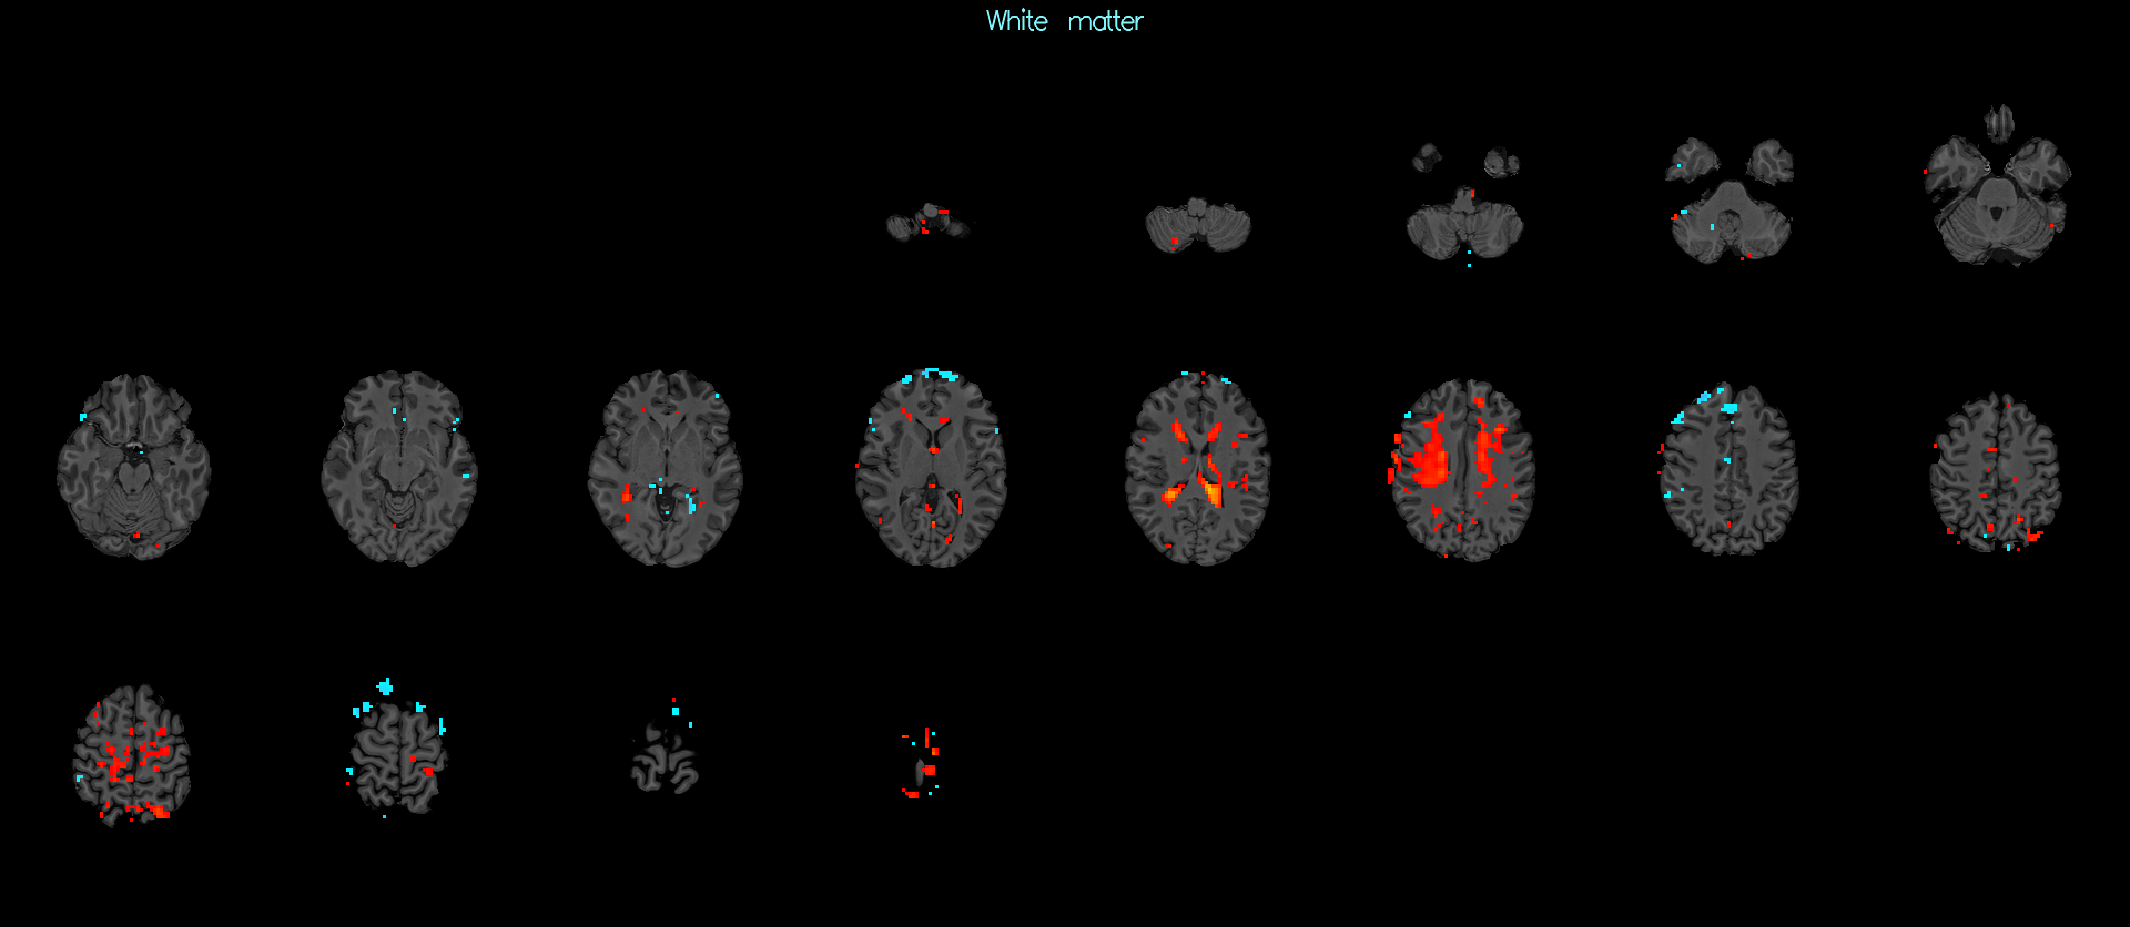
\includegraphics[width=.85\textwidth]{figures/bMethods/white_matter}  
	\caption{An example component of the white matter noise. White matter noise is visible as activation in the white matter area of the brain, while no or low activation in other regions is visible.}
	\label{fig:meth:walter_white} 
\end{figure}


\begin{figure}[H]                 
	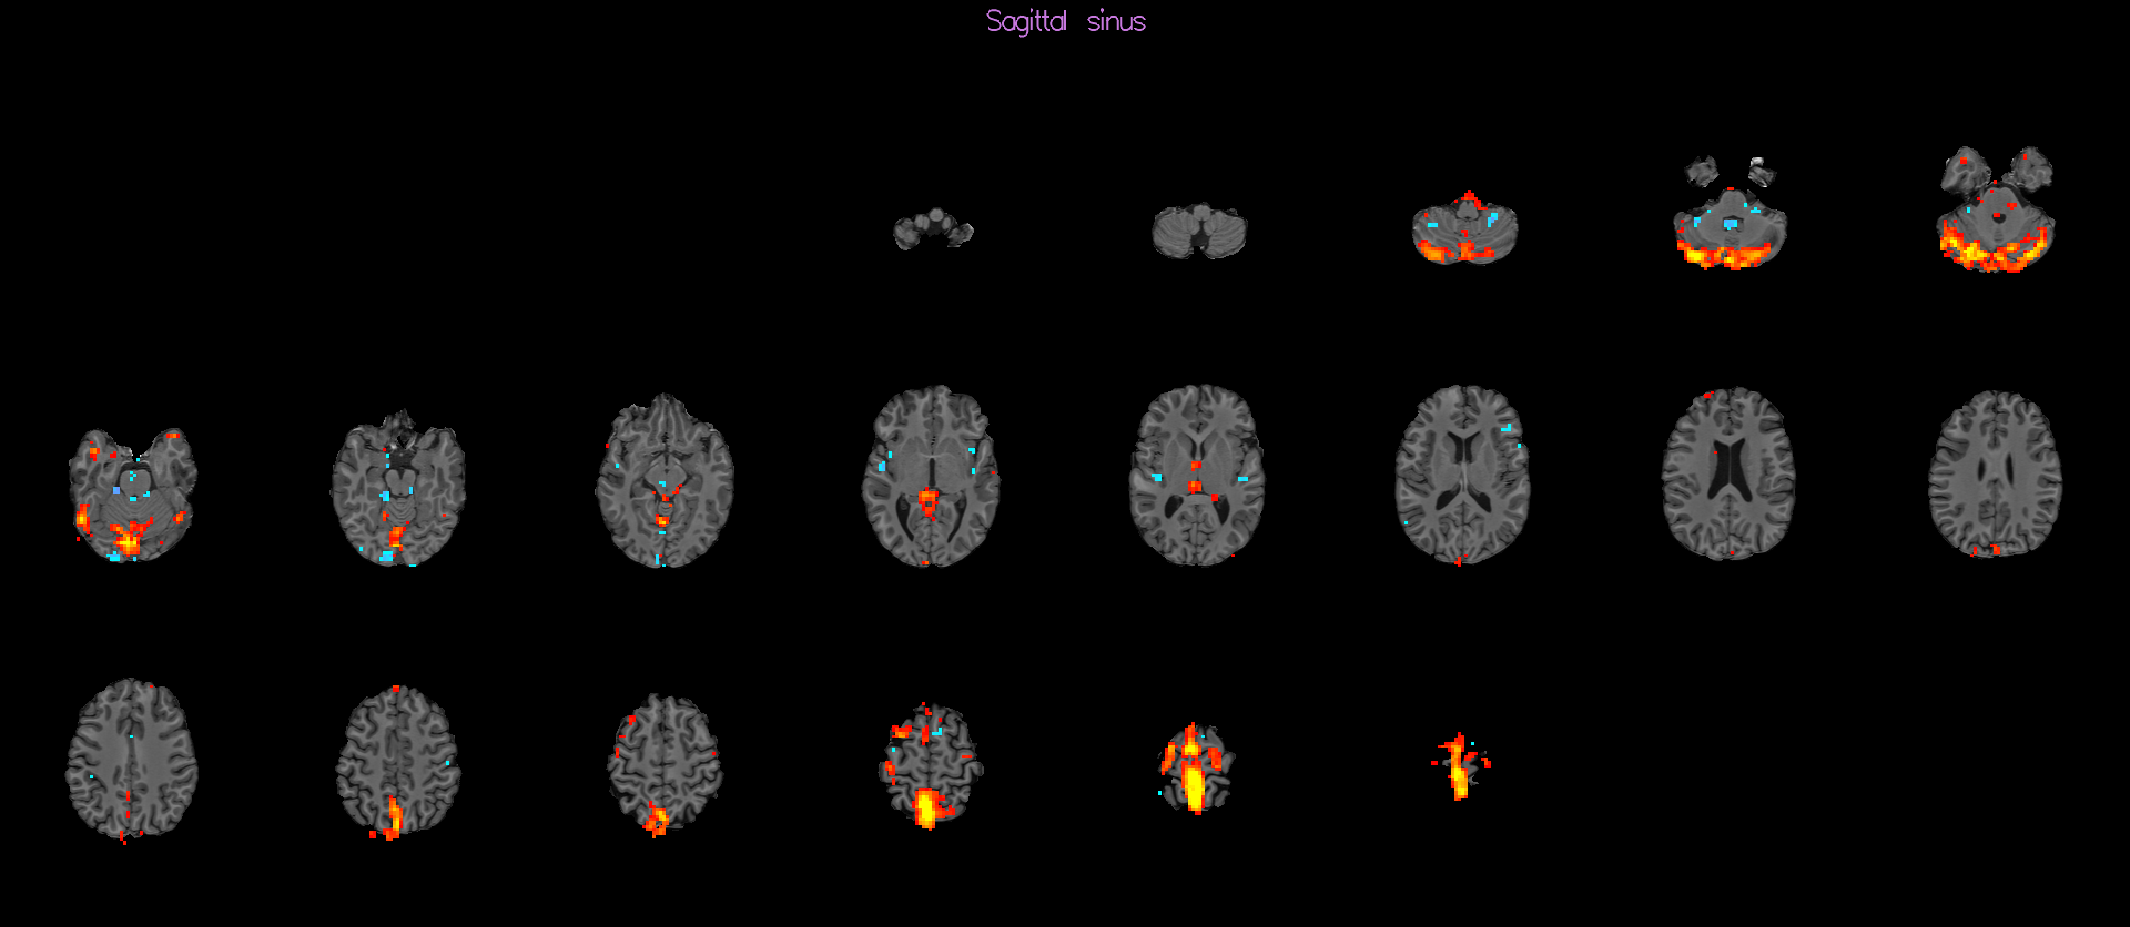
\includegraphics[width=.85\textwidth]{figures/bMethods/sag_sinus}  
	\caption{An example component of the sagittal sinus artefact. Sagittal sinus artefacts are visible as activation of the sagittal sinus veins, while no or low activation of areas of interest or noise are visible.}
	\label{fig:meth:sinus} 
\end{figure}

\begin{figure}[H]                 
	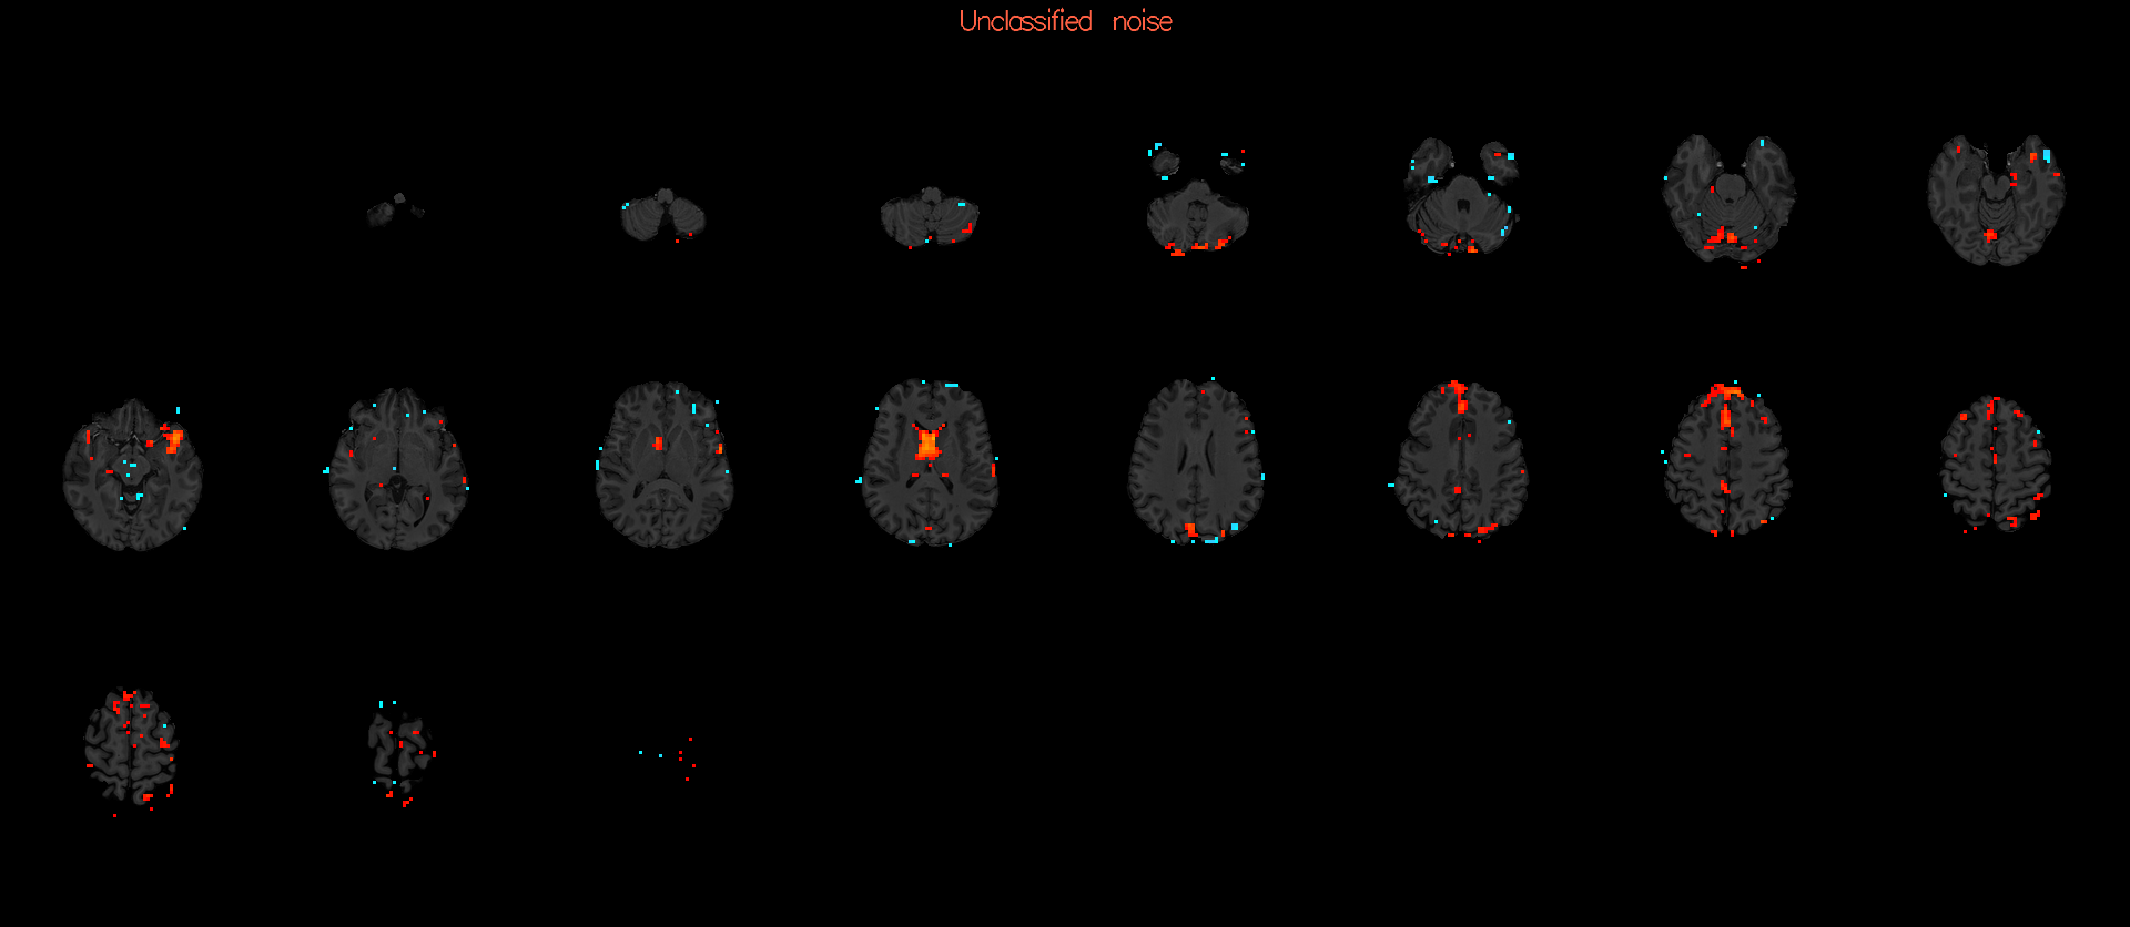
\includegraphics[width=.85\textwidth]{figures/bMethods/U_noise}  
	\caption{An example component of unclassified noise. A component was given this label when no clear noise source could be recognized and/or when the component was a mix of more than two noise sources.}
	\label{fig:meth:Unoise} 
\end{figure}


\begin{figure}[H]                 
	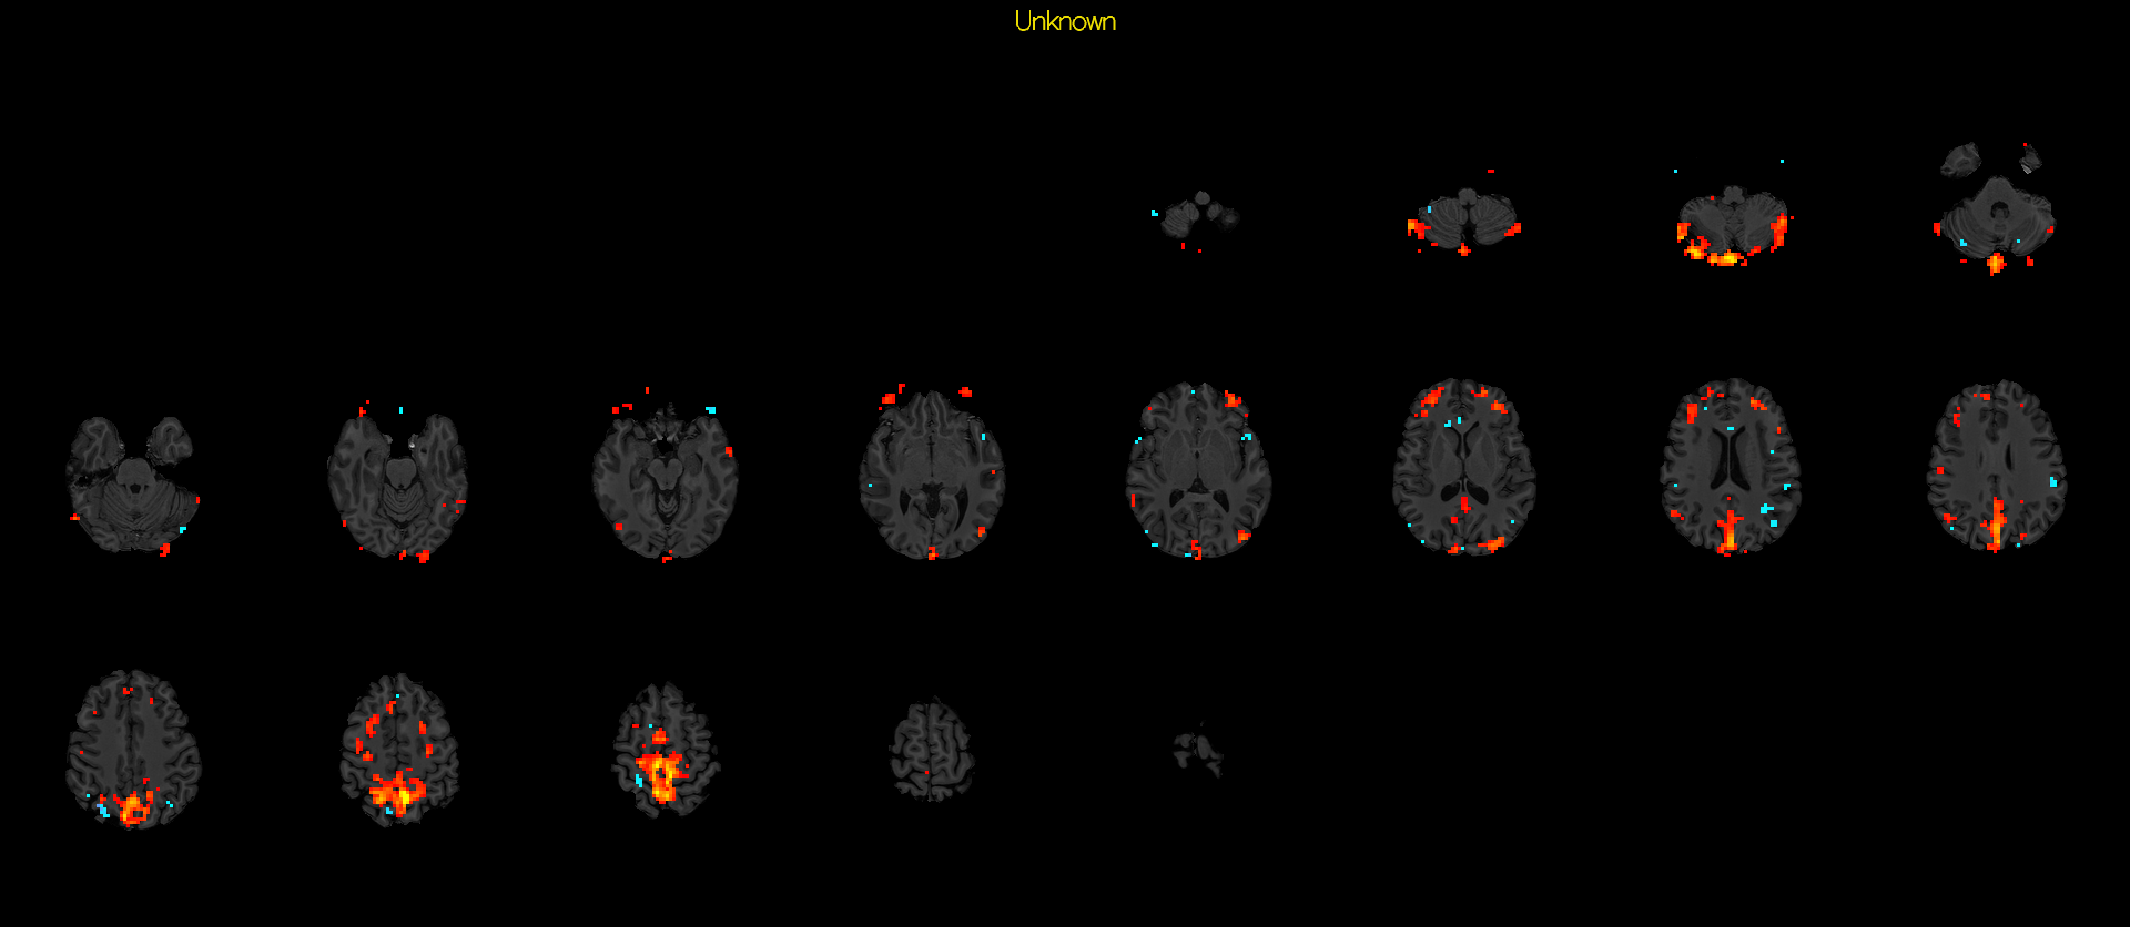
\includegraphics[width=.85\textwidth]{figures/bMethods/unknown}  
	\caption{An example component of a mix of signal of interest and noise. The signal of interest activation is either hard to localize, not seen in an expected area or the remaining spatial map is corrupted but a substantial amount of noise.}
	\label{fig:meth:unknown} 
\end{figure}

\begin{figure}[H]                 
	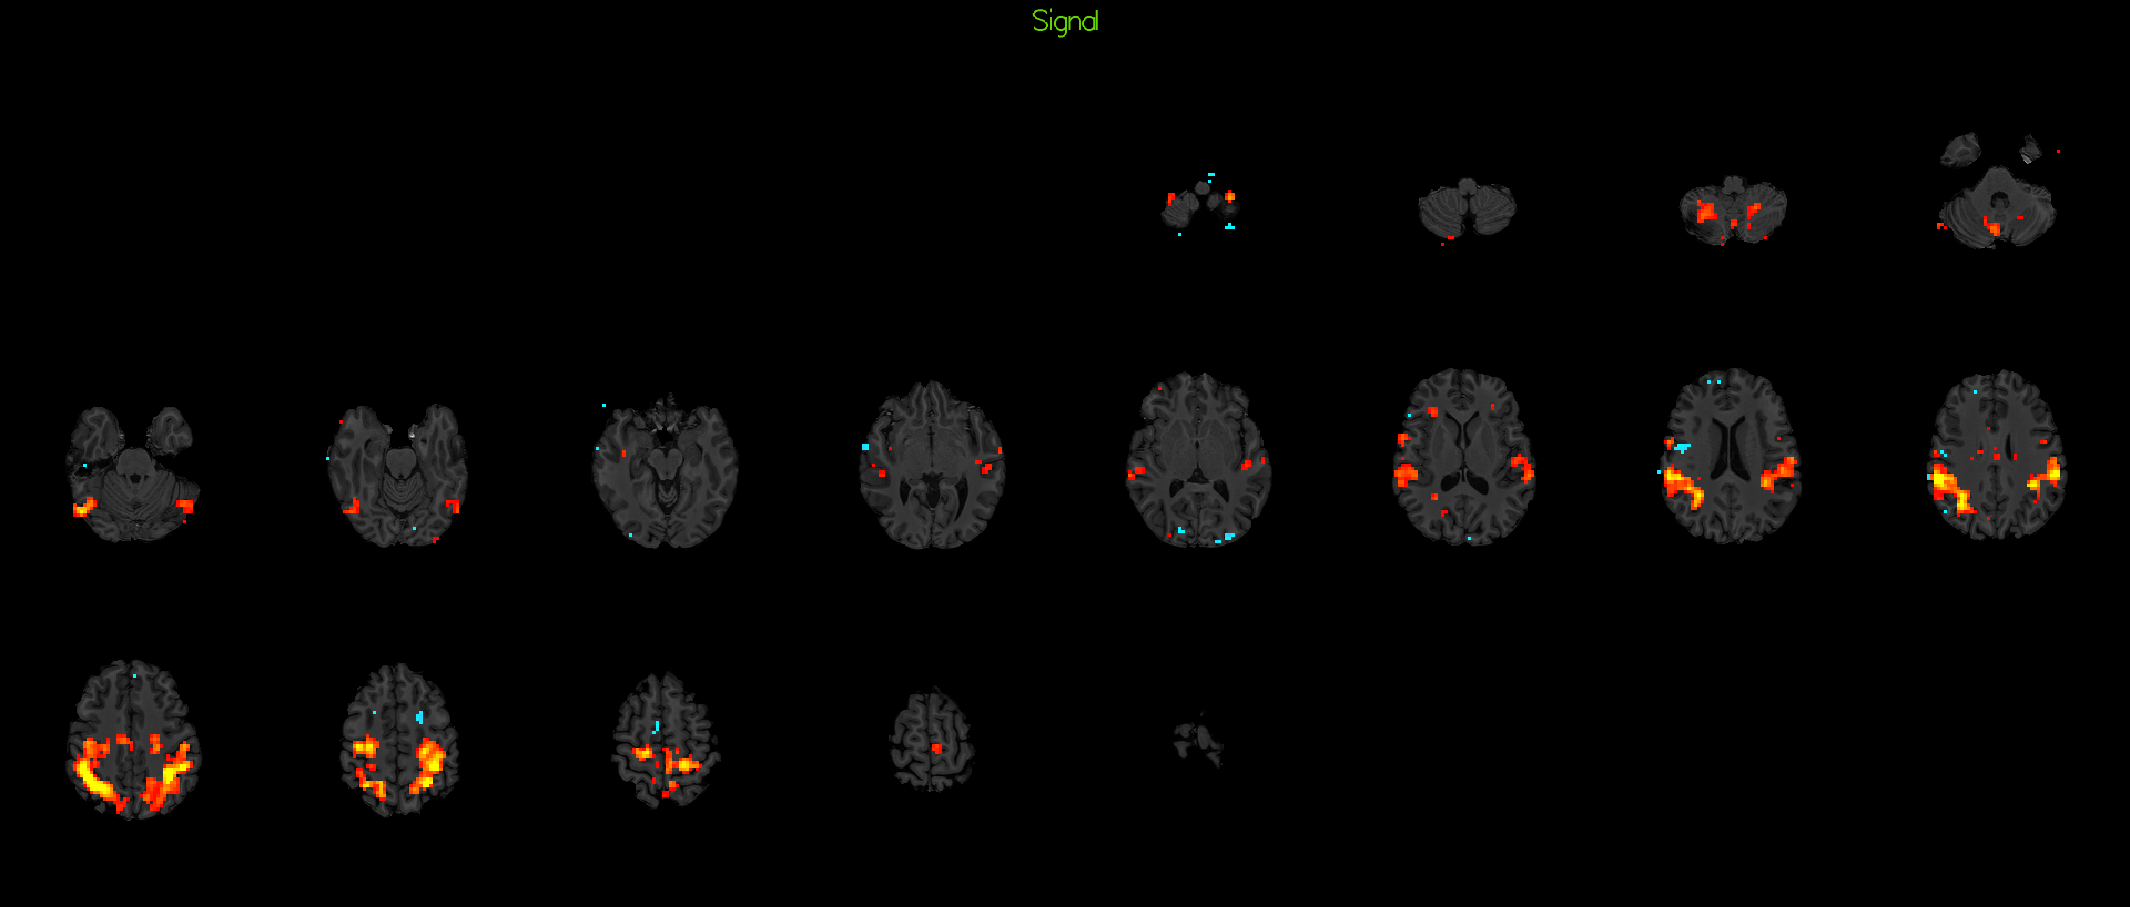
\includegraphics[width=.85\textwidth]{figures/bMethods/signal}  
	\caption{An example component of signal, which is recognizable, isolated, and not corrupted by a substantial amount of noise. In this example, the signal is characterized as a strong and fairly isolated activation mainly in the parietal lobe and temporal lobe.}
	\label{fig:meth:signal} 
\end{figure}




It should be noted that coronal and sagittal views were additionally available, along with the time course and frequency content of each components for shaping the assessment of the labeling. The corresponding structural images were used to underlay the components to assess in which brain regions the components were located. Through the component labeling the scheme, illustrated in \figref{fig:hand_label}, was used to decide whether the component was either labeled as signal, unknown or noise. 
 
 \begin{figure}[H]                 
 	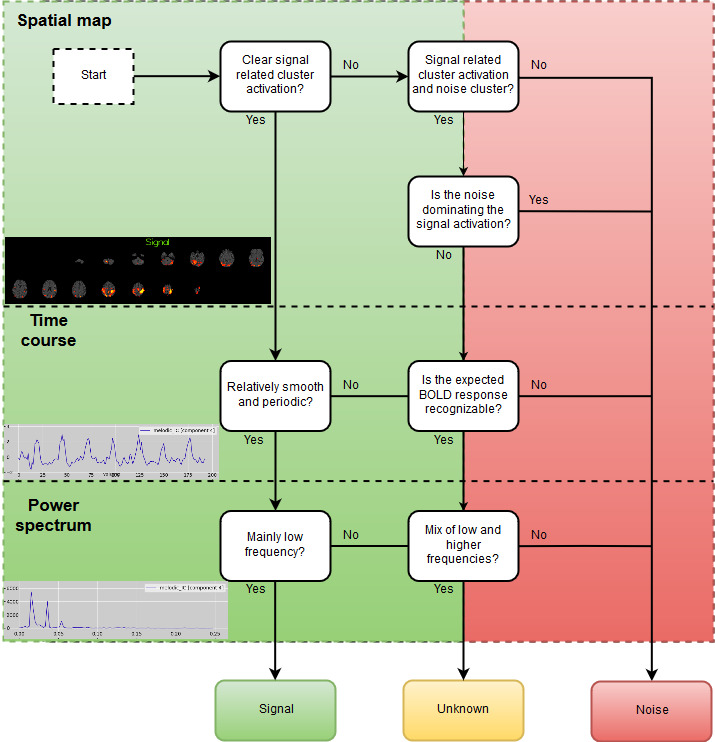
\includegraphics[width=0.85\textwidth]{figures/bMethods/Hand_labeling}  
 	\caption{A flowchart describing the assessment of a component. The component is first assessed in the spatial map, secondly the time course and lastly in the power spectrum. Note that only the assessment to either signal, unknown or noise is presented in the flowchart. When a component was found to be noise a secondary assessment into which type of noise would begin, using the information presented in \cite{Salimi-Khorshidi2014,Griffanti2017} and is therefore not accounted for in this flowchart. Illustration adapted from \cite{Griffanti2017}.}
 	\label{fig:hand_label} 
 \end{figure}
